\subsection{Product perspective}

\subsubsection{Scenarios}
Here are presented possible scenarios for the users of the S\&C platform.
\begin{enumerate}
    \item \textbf{A company wants to have access to the S\&C services:}\\
    A company would like to offer one or more internships to students, but does not know how to find/contact them and how to choose the most suitable one. Therefore, the company registers on the S\&C platform, entering its name, an email address, a password, its VAT number, contacts, a description of themselves and what it is interested in within relative fields. For subsequent times, to access it only has his/her e-mail and password.
    \item \textbf{A student wants to have access to the S\&C services:}\\
    A student wants to have the opportunity to gain more experience during his/her studies or, also, to earn some money during his/her studies and he/she doesn't know which company to choose, so he/she subscribes to the platform S\&C. When subscribing, the student enters his/her first name, last name, e-mail, a password, contacts, a description of itself and the answers to questions about his/her preferences so as to facilitate the recommendation system, within relative fields. For subsequent times, to access he/she only has to enter his/her e-mail and password.
    \item \textbf{A company insert internship offers, changes its personal data and description}\\
    Now that it is inside the platform, the company can add its new internship offer, inserting the title, an adequate description, the characteristics and the questions to be included in the relative form that will be filled out by the student at the beginning of the selection process. Or it can modify/update existing offers, its personal data and descriptions.
    \item \textbf{A student insert his/her CV, changes his/her personal data, descriptions and preferences}\\
    Now that it is inside the platform the student can insert or modify his/her CV by uploading it as a PDF. He/She can also modify/update his/her personal data and description.
    \item \textbf{A student search for an internship}\\
    To search for an internship, the student must enter a keyword or the name of a company in the search bar, and can customize his/her search through filters. Once he/she has chosen the offer that is right for him/her, he/she can request to start the selection process and S\&C will take care of notifying the company in question.
    \item \textbf{Recommendation system notification}\\
    Based on the preference inserted by the student and the companies and the statistical analysis from the data collected by the platform, they get notified when a match is available, throughout the research made by the recommendation system.
    \item \textbf{Acceptance phase}\\
    When the student or the company receive a notification, they have to accept or refuse it through a button. if they accept they must indicate their availability spots and the platform will find the first free spot in common for the video interview. If that does not exists notify both with their e-mail.
    \item \textbf{Selection process}\\
    After the establishment of a contact, the selection process start, and the student has to compile a form with specific questions to check if he/she really fit with the position. Then they proceed with the scheduled interview through a Zoom link provided by the platform. After the interview, both participant can accept or not the collaboration.
    \item \textbf{Ending internship}\\
    At the end of the internship the student and the company can leave feedback on the counterpart.    
\end{enumerate}

\subsubsection{Domain-level Diagram}
\begin{figure}[H]
    \centering
    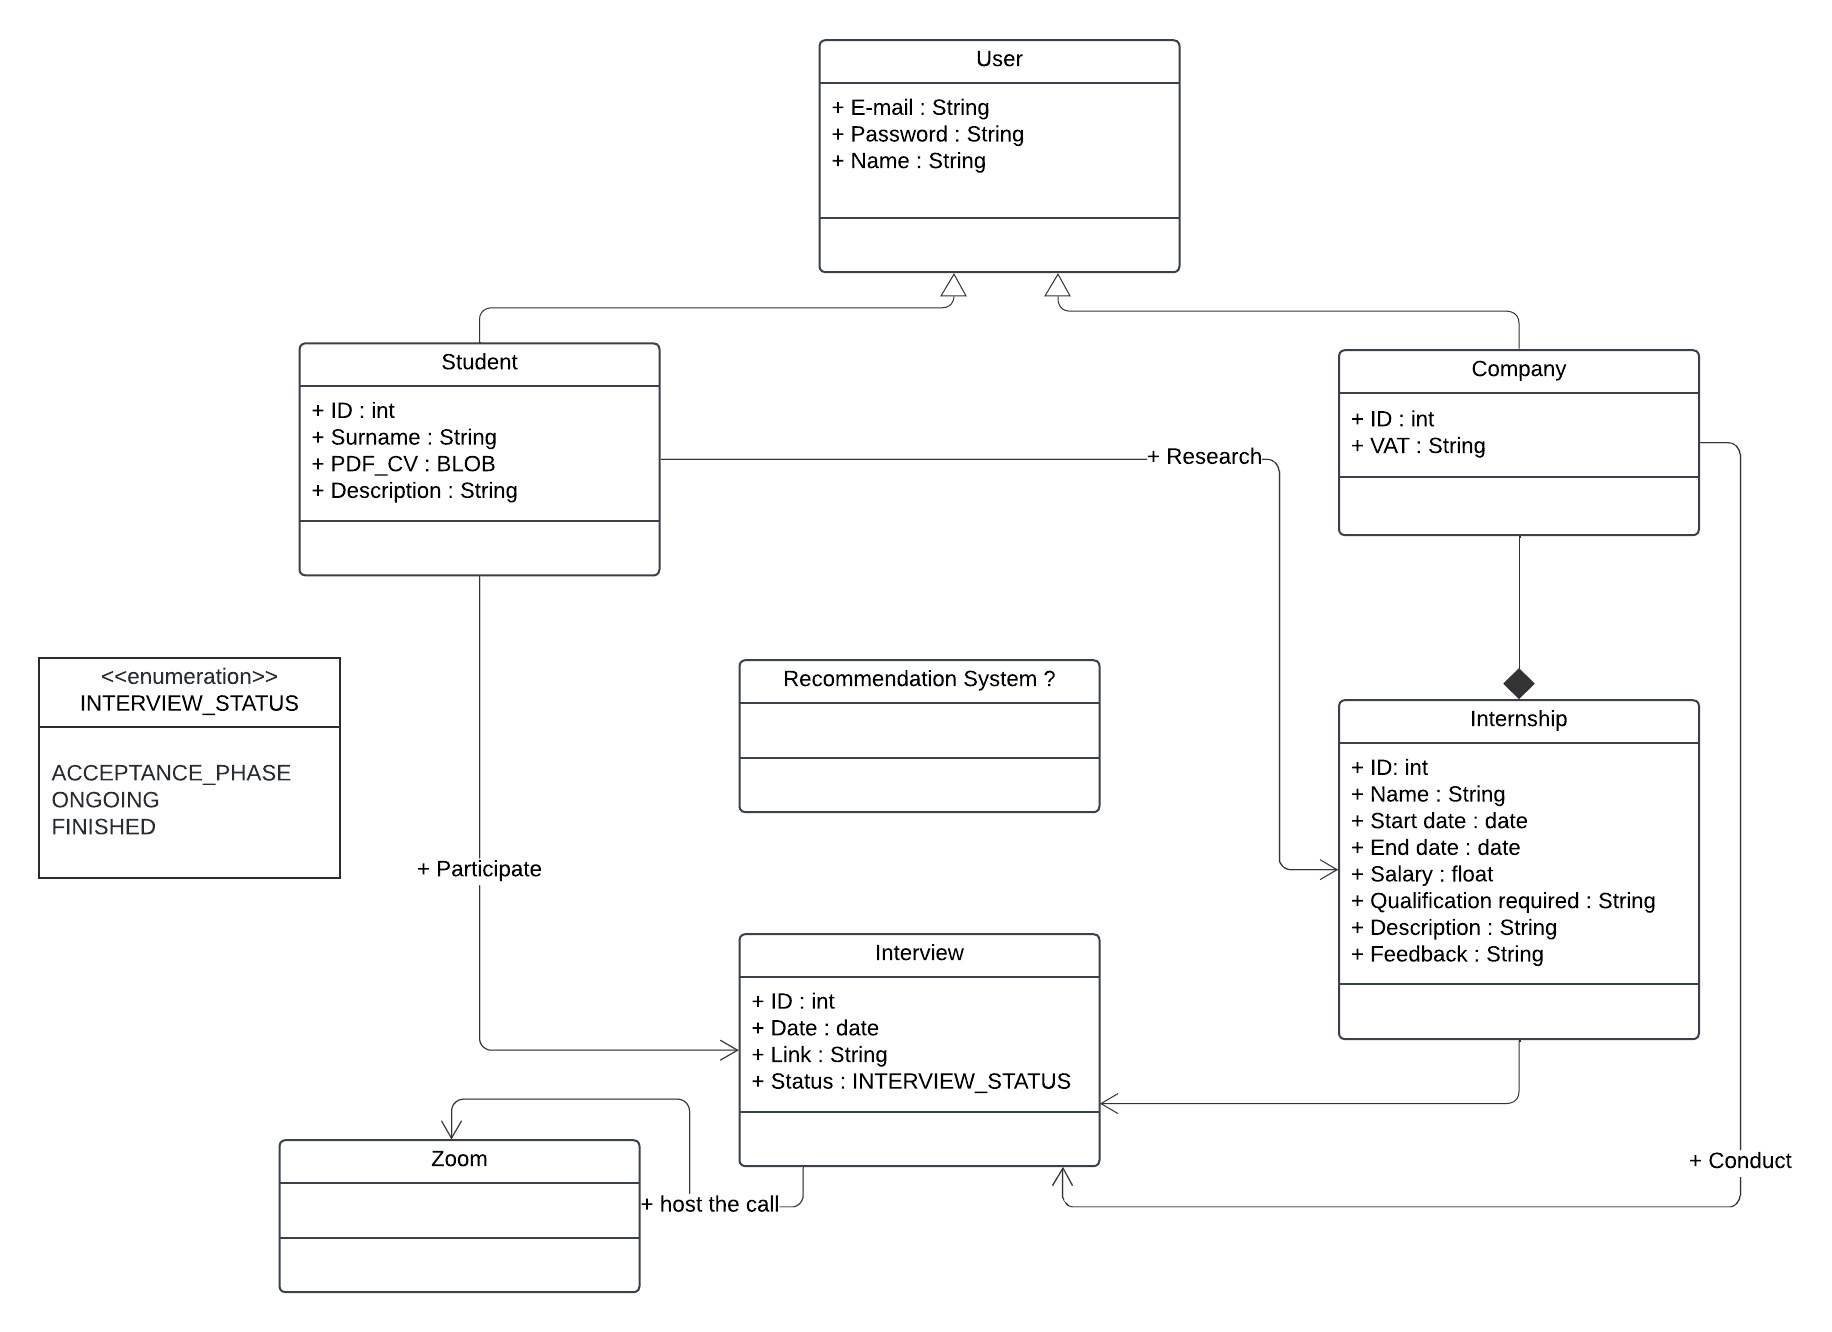
\includegraphics[width=\textwidth]{Images/Class diagram.png}
    \caption{Class diagram}
    \label{Class diagram}
\end{figure}

\subsubsection{State Diagrams}
State diagrams describe the behavior of the system while considering all possible states the system can deal with when an event occurs. This analysis helps to clarify the most critical aspects of the system.
\begin{figure}[H]
    \centering
    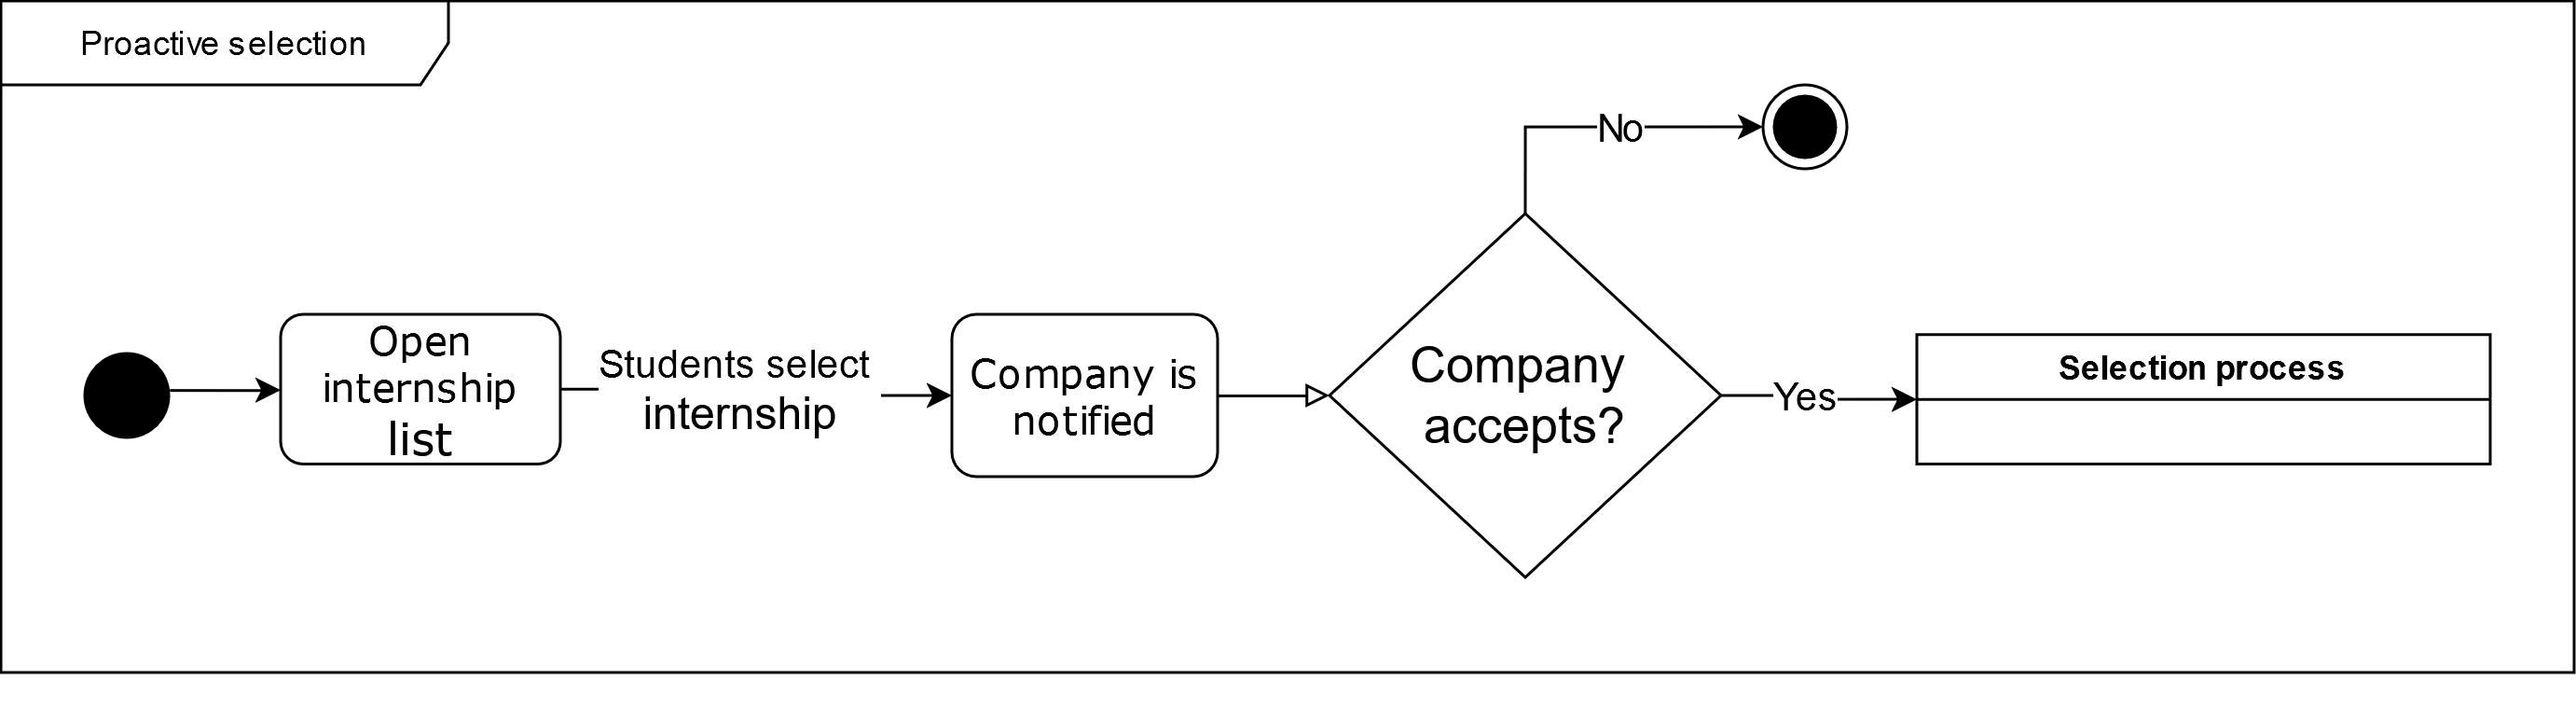
\includegraphics[width=\textwidth]{Images/Proactive selection.png}
    \caption{Proactive selection}
    \label{Proactive selection}
\end{figure}
This state diagram describes the process of manual selection of the internship by the student. In the initial state, the "Open internship list" the system is displaying some internship, and the student can select one of them, when is selected the system goes into the "Company is notified" state and notify the company interested, that can accept or not the request, in case of acceptance, the selection process start. 
\begin{figure}[H]
    \centering
    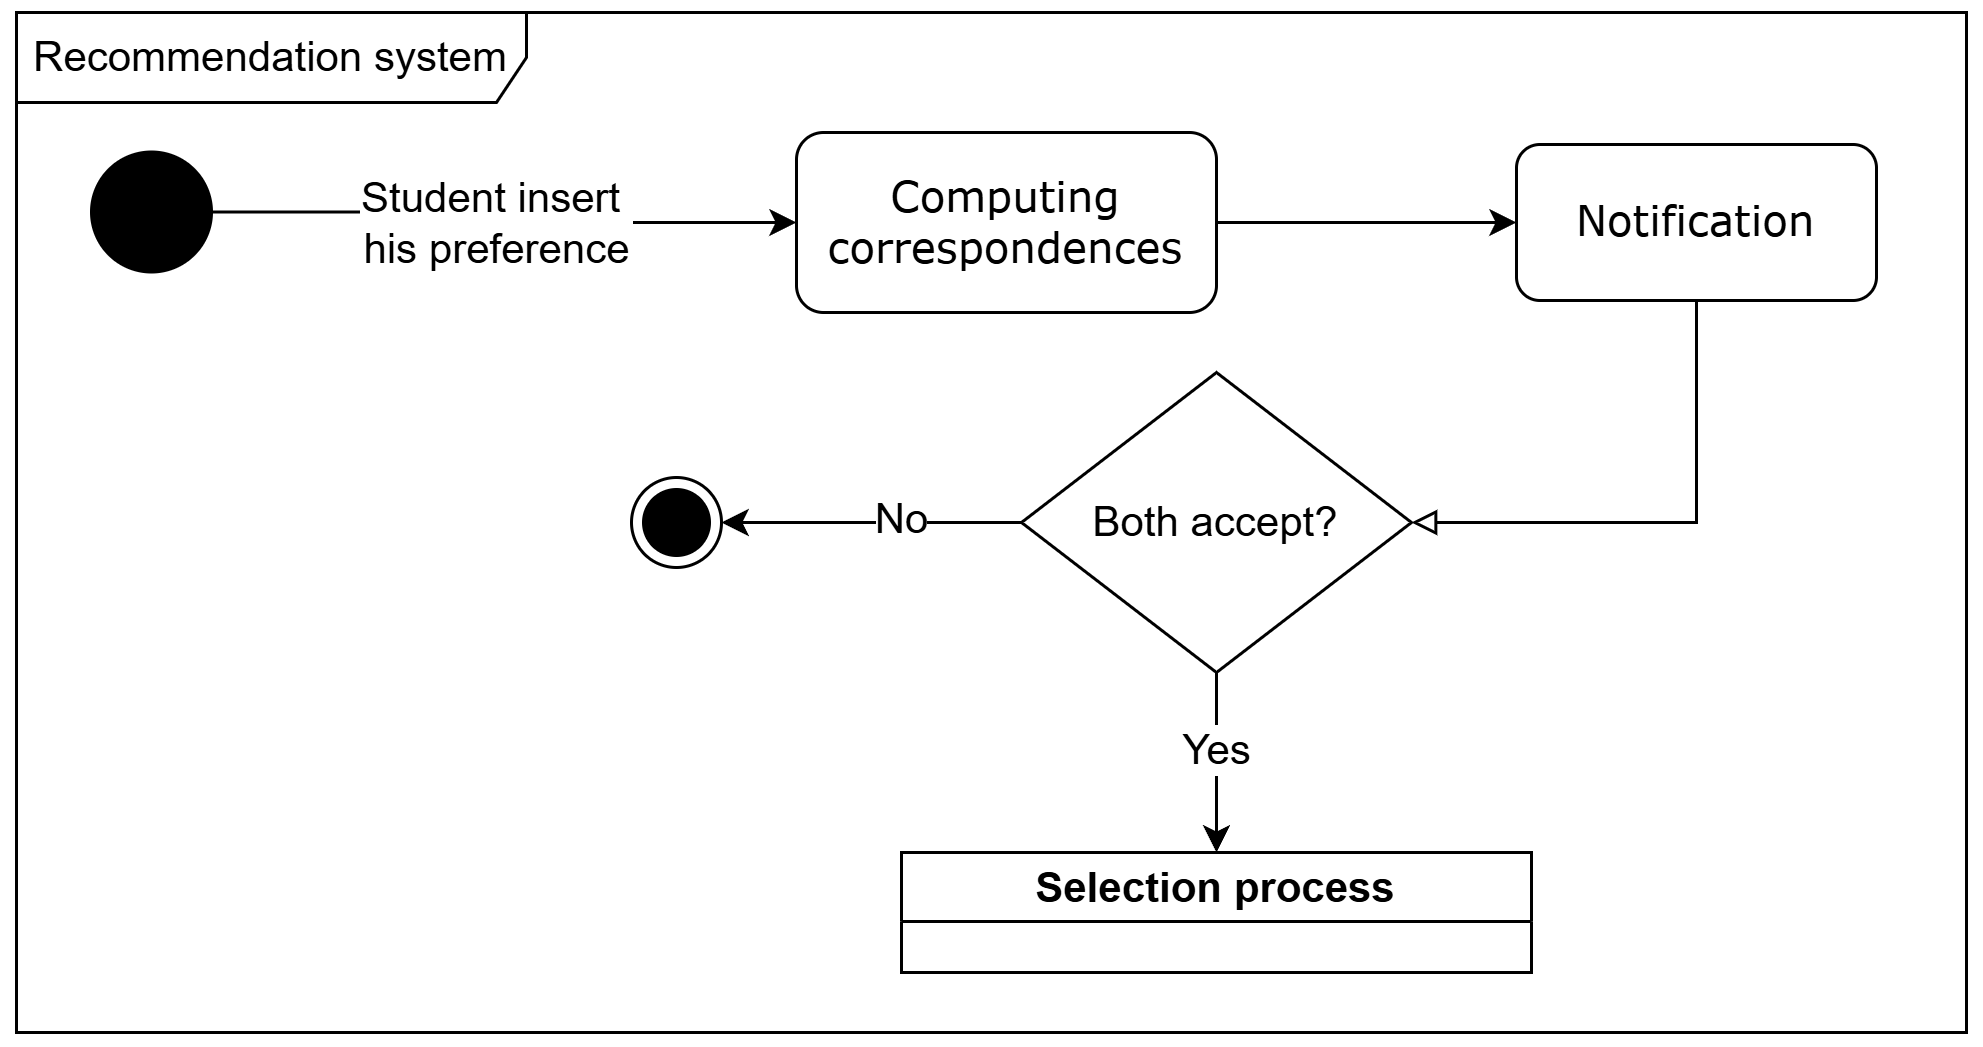
\includegraphics[width=\textwidth]{Images/Recommendation system.png}
    \caption{Recommendation process}
    \label{Recommendetion system}
\end{figure}
After the insertion of the preferences by the student, the system goes to the state of "computing correspondences" where it actually search for an internship that can match with the preferences of a company, through a keyword search of the preferences through the CVs' content or a statistical analysis of the internships. The system always found the best match, then proceed to the state of "notification" where it notify both the counterparts, if both of them accept, then the system proceed with the selection process, else the selection process never start.
\begin{figure}[H]
    \centering
    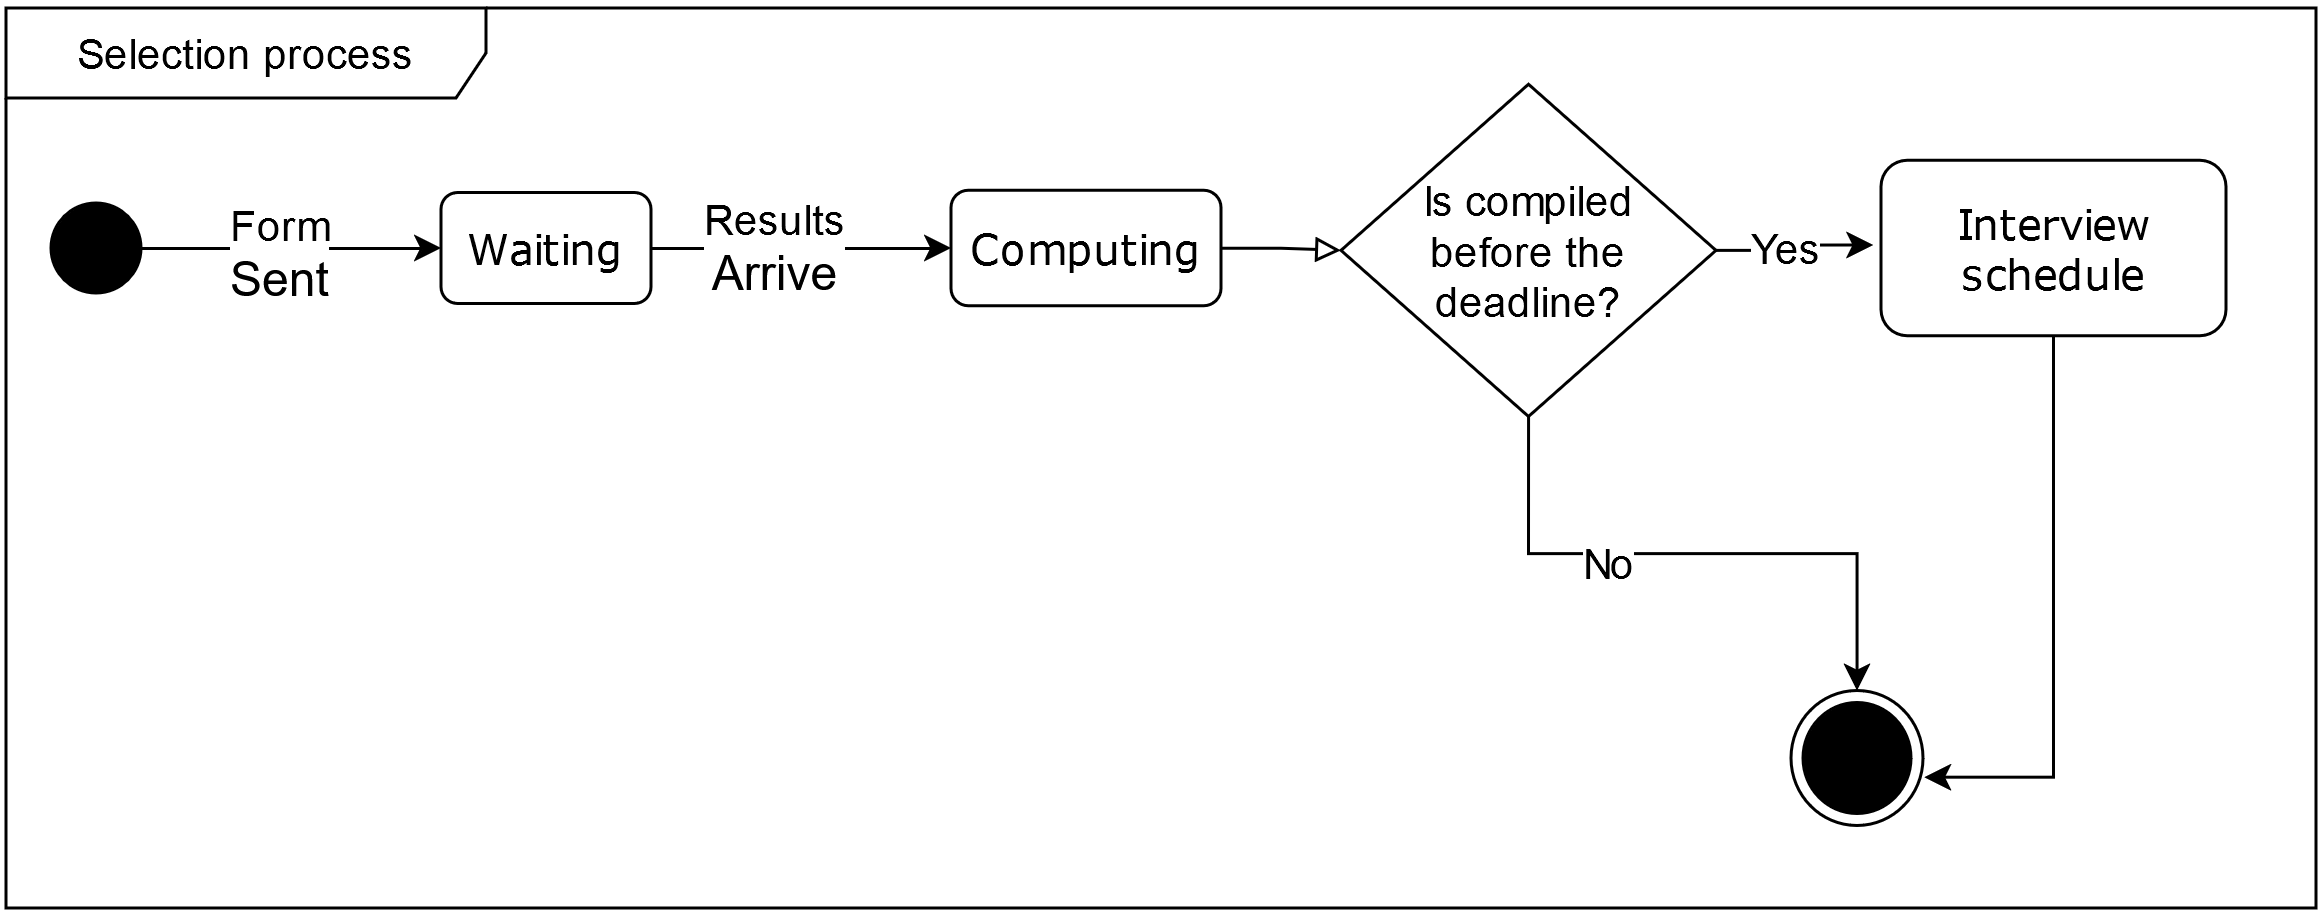
\includegraphics[width=\textwidth]{Images/Selection process.png}
    \caption{Selection process}
    \label{Selection process}
\end{figure}
This state diagram describe the selection process, once it starts, the system sent a form and goes to the "Waiting" state, where it waits until the student compile the form and send back the results, Then when they arrive, it goes to the "Computing" state and elaborate the form result and if the date of compiling is before the deadline, the system proceeds with the scheduling of the interview in the "Interview schedule" state, where it also produce the link for the video interview. 

\subsection{Product functions}
The following sections contains the main product function of S\&C.
\begin{itemize}
    \item \textbf{Sign and Login}\\
    These functions will be available to all the users. The sign-up functionality allows users to create an account to register themselves to the platform. Each user will be asked to select if he/she is a student or a company and provide own data such as name, email and password; for the student will also be asked surname, his/her description and CV, for the company the VAT number and a description of itself. The login functionality allows users to access an existing account using the credentials (email and password) chosen at registration. 
    \item \textbf{Managing internships and data}\\
    This function allows companies to insert their offers into the platform, it requires a name, a start and an end date, if there is one, a salary, the qualification required and a description. Also a company can modify the existent one and its data.
    \item \textbf{Managing student data}\\
    This function allows a student to insert his/her updated data.
    \item \textbf{Autonomous research}\\
    This function allows a student to search throughout all the internships available and find what suits him better and he/she ask the company to start the selection process. He/She can search through the list with a keyword or through the application of some filter. 
    \item \textbf{Recommendation system}\\
    This function search for a correspondence between the student and the companies, taking in consideration the CV of the student, the preferences and the description of both. If this search fails, it takes in consideration a statistical analysis approach that produce the most suitable match from the list of internships.
    \item \textbf{Selection process}\\
    This function handle the selection process, once all the parts have accepted to collaborate, S\&C sends a form to the student, and when the student send it back, it check if it has done in time, if yes, schedules an interview for the first spot available for both the student and the company, else it ends the process. The function will end after the acceptance or not by the company of the student after the interview. 
\end{itemize}

\subsection{User characteristics}
Here it is provided a more detailed characterization of the two different types of users of the platform, also specifying the roles they can assume in different contexts. 
\begin{itemize}
    \item \textbf{Student}\\
    A student can be whoever wants to search for an internship and his/her is a real university student. After his/her registration, he/she gets the functionalities which are reserved for student such as managing data and autonomously searching for an internship.
    \item \textbf{Company}\\
    A company can be whoever wants to offer an internship. After its registration, it gets the functionalities which are reserved for companies such as managing data and offers for an internship.
\end{itemize}

\subsection{Assumptions, dependencies, and constraints}
\textbf{[A1]:} The user always selects the correct option about his/her/its position (student/company)\\
\textbf{[A2]:} All users have an active email address.\\ 
\textbf{[A3]:} All users have access to an internet connection\\
\textbf{[A4]:} A student is a real student, subscribed to a University.\\
\textbf{[A5]:} All users have a Zoom account.\\
\textbf{[A6]:} All Companies are real companies, and the inserted VAT number can be verified.\\
\textbf{[A7]:} The internship should start from a valid date, which is later from the interview date




Here is the command to refer to another element (section, figure, table, ...) in the document: \emph{As discussed in Section~\ref{sect:overview} and as shown in Figure~\ref{fig:metamodel}, ...}. Here is how to introduce a bibliographic citation~\cite{DAM}. Bibliographic references should be included in a \texttt{.bib} file.